\section{Task 1: Data audit and retained trip counts}
\label{sec:task1}
We audited all 51,043,773 recorded trip rows from the four TLC files using the official data dictionaries and zone lookup. Pickup timestamps determine month membership across source files. The completed-trip count set requires pickup and dropoff timestamps, pickup in April--May 2026, and a positive timestamp duration. Zone, distance, payment, and sharing rules are applied only to analyses that require those fields. This avoids treating missing monetary components as zero or removing valid trip records from a count solely because a non-count field is anomalous.

The audit found 1,117,613 records with at least one reported flag and 581,595 with two or more flags. These are diagnostic flags rather than a universal exclusion count. Detailed rule counts, pairwise overlaps, retained samples, and example records are supplied in the Task 1 CSV supplements. Extreme distance above 100 miles is retained in trip counts and OD volumes but excluded from distance-dependent analyses. Passenger spending above \$1,000 is reviewed but not automatically removed from spending summaries.

\begin{table}[htbp]
\centering\small
\caption{Selected audit flags across all four raw files. Counts overlap and are not additive.}
\begin{tabular}{lr}
\hline
Audit flag & Records \\
\hline
on scene order invalid & 765,096 \\
request after pickup & 544,494 \\
distance nonpositive & 210,688 \\
duration nonpositive & 101,574 \\
payment negative & 34,345 \\
distance gt100mi & 4,040 \\
shared ny & 1,960 \\
\hline
\end{tabular}
\end{table}

The request-after-pickup and on-scene-order flags overlap for 544,494 records. For Task 1.2, 50,942,185 trips are retained. Field-specific retention for later analyses is reported separately in the CSV supplement.

\begin{table}[htbp]
\centering\small
\caption{Retained recorded trips by all four named HVFHV licenses and request/match status. Flags are ordered request first, match second; zeros are explicit.}
\begin{tabular}{lllrr}
\hline
License & Service & Request/match & April & May \\
\hline
- & Yellow taxi & All retained trips & 3,781,728 & 4,038,760 \\
- & HVFHV & All retained trips & 20,995,953 & 22,125,744 \\
HV0002 & Juno & N/N & 0 & 0 \\
HV0002 & Juno & Y/N & 0 & 0 \\
HV0002 & Juno & Y/Y & 0 & 0 \\
HV0002 & Juno & N/Y & 0 & 0 \\
HV0002 & Juno & Missing/other & 0 & 0 \\
HV0002 & Juno & All retained trips & 0 & 0 \\
HV0003 & Uber & N/N & 14,961,455 & 14,966,066 \\
HV0003 & Uber & Y/N & 162,018 & 167,846 \\
HV0003 & Uber & Y/Y & 255,385 & 220,904 \\
HV0003 & Uber & N/Y & 0 & 0 \\
HV0003 & Uber & Missing/other & 0 & 0 \\
HV0003 & Uber & All retained trips & 15,378,858 & 15,354,816 \\
HV0004 & Via & N/N & 0 & 0 \\
HV0004 & Via & Y/N & 0 & 0 \\
HV0004 & Via & Y/Y & 0 & 0 \\
HV0004 & Via & N/Y & 0 & 0 \\
HV0004 & Via & Missing/other & 0 & 0 \\
HV0004 & Via & All retained trips & 0 & 0 \\
HV0005 & Lyft & N/N & 5,614,374 & 6,767,729 \\
HV0005 & Lyft & Y/N & 1,865 & 1,954 \\
HV0005 & Lyft & Y/Y & 73 & 68 \\
HV0005 & Lyft & N/Y & 783 & 1,177 \\
HV0005 & Lyft & Missing/other & 0 & 0 \\
HV0005 & Lyft & All retained trips & 5,617,095 & 6,770,928 \\
\hline
\end{tabular}
\end{table}

For Juno (HV0002), Uber (HV0003), Via (HV0004), and Lyft (HV0005), each company subtotal equals its five status rows. The four subtotals, plus any separately reported other company codes, reconcile exactly to the HVFHV retained total in each month. Juno and Via have zero retained records in both study months. The N/Y status is retained as a reporting-inconsistency category, while missing or other flag statuses are listed separately. Counts refer to records of observed completed trips, not distinct people, vehicles, or all travel requests. Yellow taxi has no specified sharing status, so it is not subdivided by sharing flags.

% Task 1 visualizations
\begin{figure}[htbp]\centering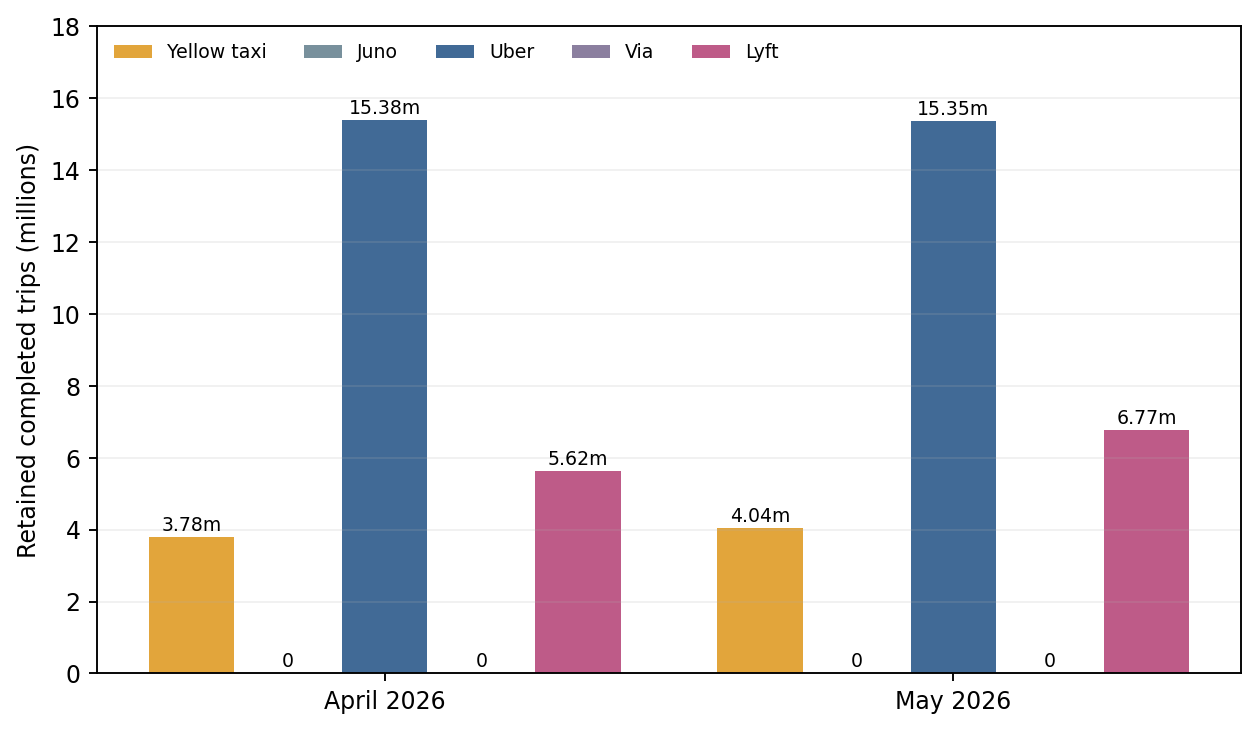
\includegraphics[width=.68\textwidth]{04_Results/Task_1/figures/retained_trips_by_service.png}
\caption{Retained completed trip records by month and service. Juno (HV0002) and Via (HV0004) have zero records; all four named HVFHV companies reconcile to the HVFHV total.}\label{fig:t1service}\end{figure}
\begin{figure}[htbp]\centering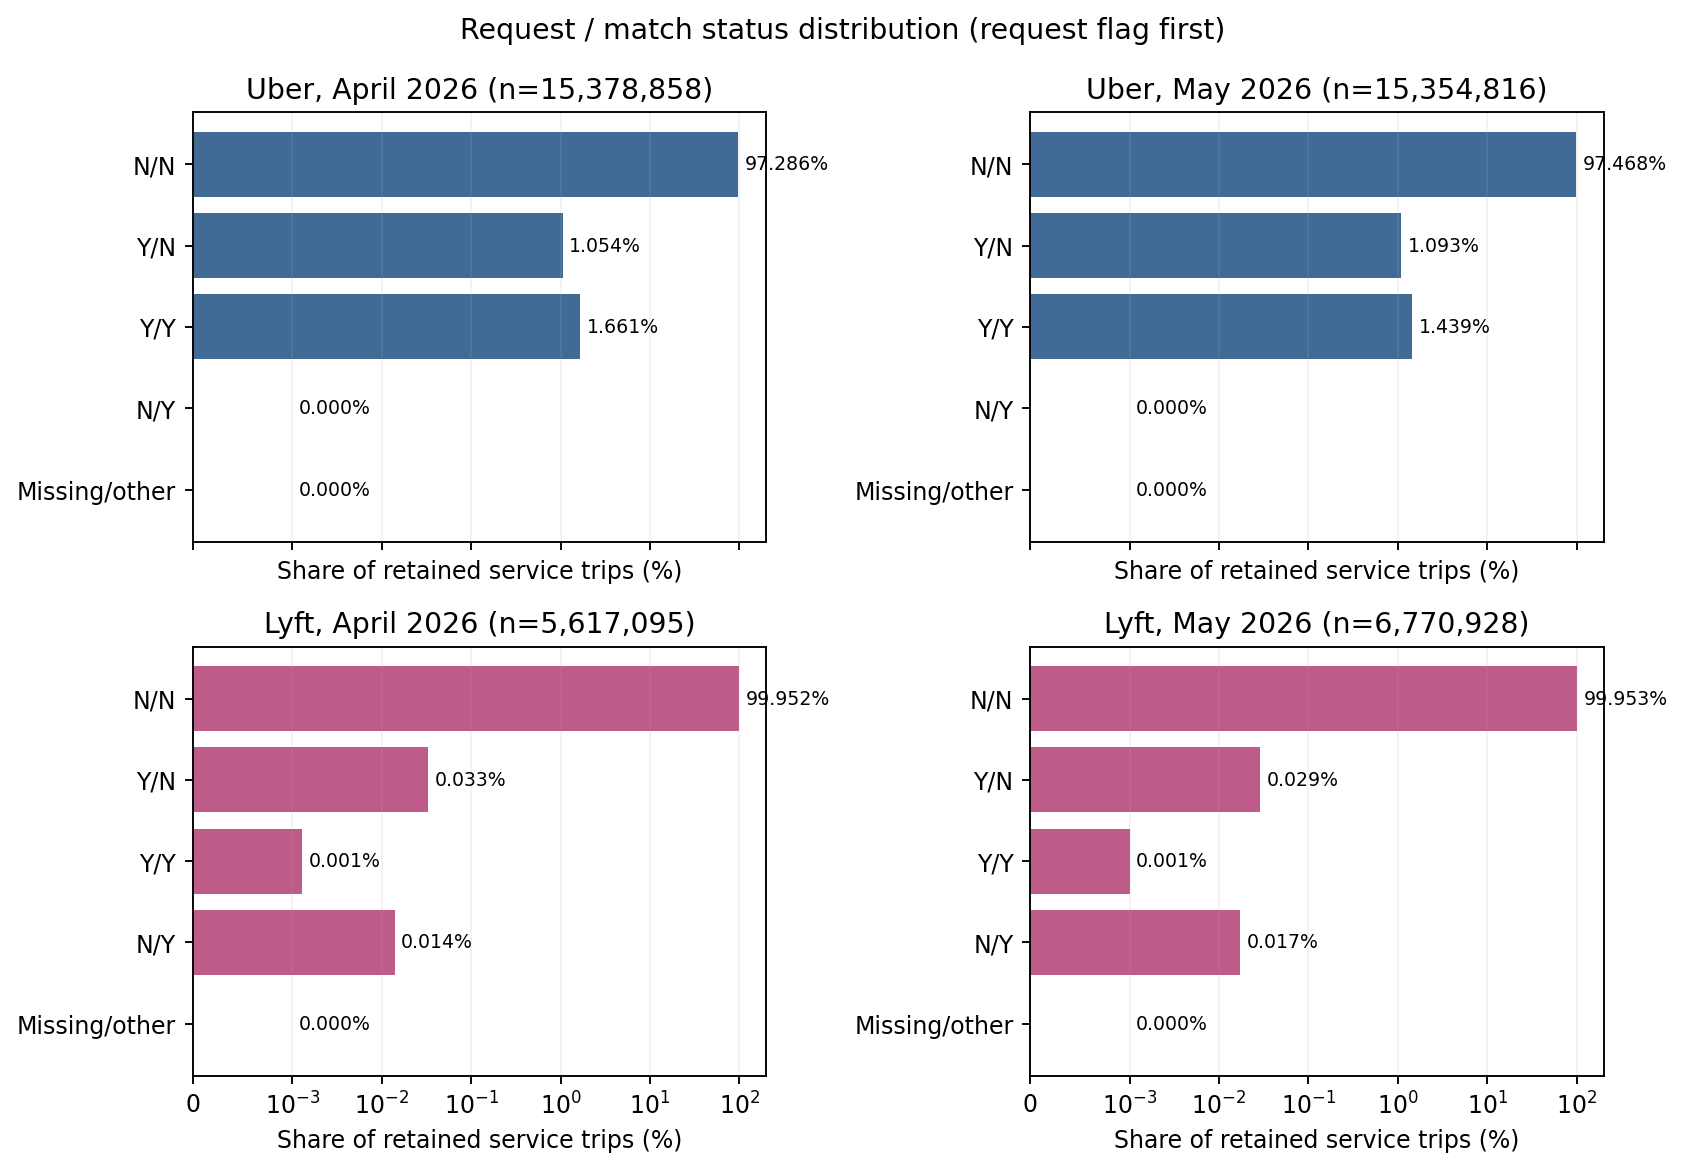
\includegraphics[width=.83\textwidth]{04_Results/Task_1/figures/sharing_status_distribution.png}
\caption{Request/match categories for the two companies with retained records, Uber and Lyft. Juno and Via have zero denominator, so shares are undefined. The symmetric log axis preserves visibility of rare statuses and zero values.}\label{fig:t1status}\end{figure}
\begin{figure}[htbp]\centering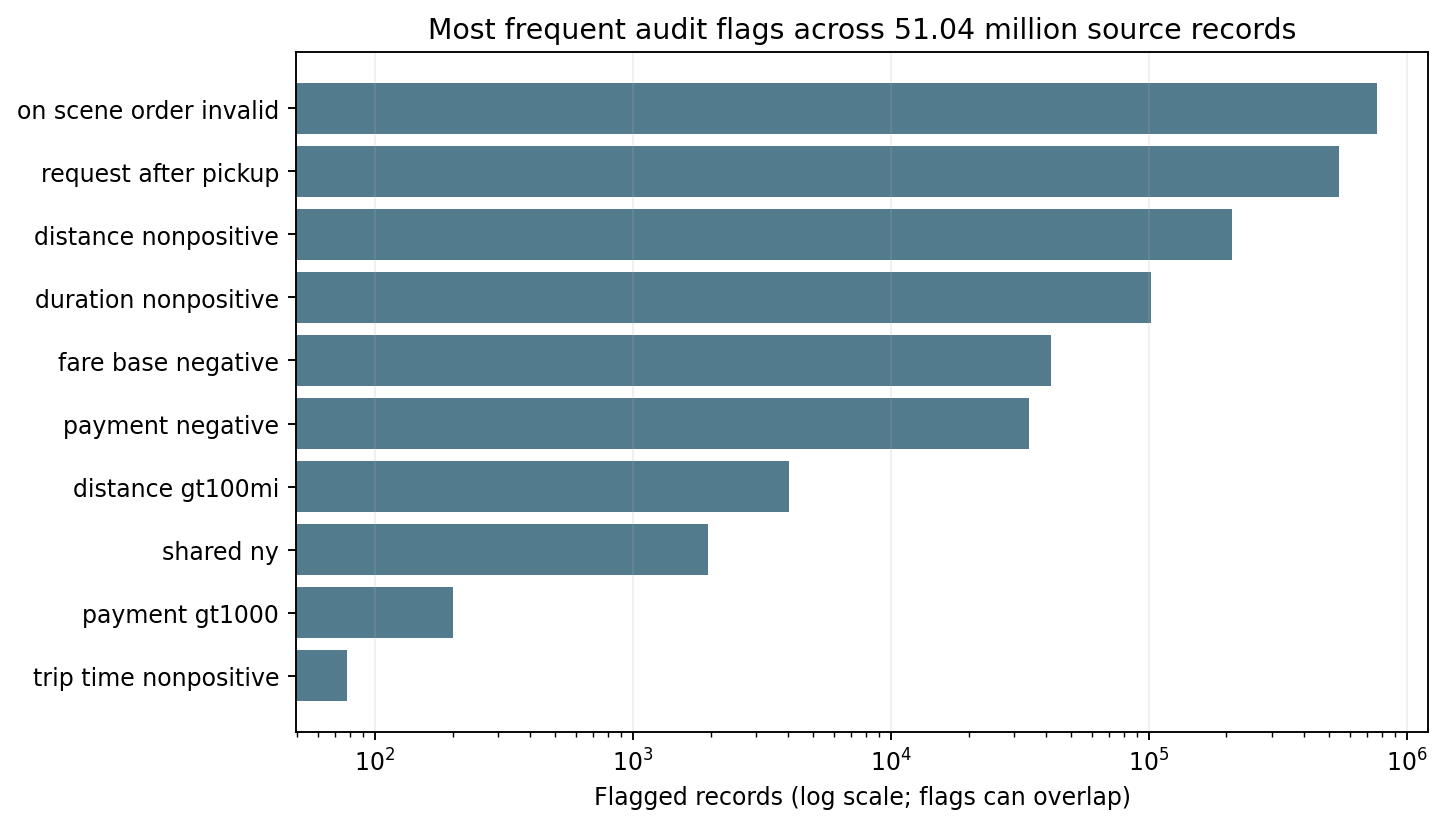
\includegraphics[width=.73\textwidth]{04_Results/Task_1/figures/audit_flags.png}
\caption{Most frequent diagnostic flags. Flags overlap, so bar lengths must not be added.}\label{fig:t1audit}\end{figure}
